\documentclass{article}
\usepackage{amsmath, amssymb, graphicx, verbatim}
\usepackage[margin=1in]{geometry}
\title{CMPS 142: Homework Assignment 3}
\author{Jeffrey Petersen - 1329242\\Ben Gordon - 1263760\\Raymond Colebaugh - 1377877}
\begin{document}
\maketitle
\begin{enumerate}
        \item 
	    We want to find the minimum of the geometric margin, \[min_{w,b} \frac{y(w \cdot x_{i} + b)}{||w||^2}\]
	    Our decision boundary will be of the form \(w \cdot{x_{i}}+b > 0 \), which can also be expressed as \(w_{1}x + w_{2}y + b > 0\).
	    After graphing the data and evaluating them visually, we can find a good candidate for a decision boundary at \(y>-x+\frac{3}{2}\),
	    or \(x+y-\frac{3}{2}>0\). Our \(w_{1}\) and \(w_{2}\) are both 1 and we have a margin of \(\frac{2}{||w||} = \sqrt{2}\). 
	    The support vectors, then, are (1,1), (1,0), and (0,1).
        \item
            In executing grid search with the specified bounds on parameters, we
            determined the following costs and gammas for SMO:
            $$ \begin{tabular}{c c c c c c c | c c c}
                $C_{ min }$ & $C_{ max }$ & $C_{ step }$ & $\gamma_{ min }$ & $\gamma_{ max }$ & $\gamma_{ step }$ & Sample Size & C & $\gamma$ & Accuracy \\ \hline
                1    &   16    &    1     &       -5     &     2        &        1         &  25\%    &  16 & 0 & 93.6318 \%   \\
                1    &   16    &    1     &       -5     &     2        &        1         &  50\%    &  14 & 1 & 93.6101 \% \\
                15    &   32    &    1     &       0     &     2        &        0.25      &  10\%    &  31 & 0 & 93.6536 \%  \\
                15    &   32    &    1     &       0     &     2        &        0.25      &  25\%    &  25 & 0 & 93.697 \%  \\
                23    &   27    &    0.25  &       0.7   &     1.3      &        0.1       &  10\%    &  27 & 0.7  & 93.3275 \% \\
                23    &   27    &    0.25  &       0.7   &     1.3      &        0.1       &  25\%    &  25.75 & 0.7 & 93.371 \% \\
                23    &   27    &    0.25  &       0.7   &     1.3      &        0.1       &  50\%    &  24.75 & 0.7 & 93.371 \%
            \end{tabular} $$
            Where the expression for $c$ was $i$ and the expression for $\gamma$ was $10^i$. Whenever one of the parameters was chosen
            to be on a boundry, such as the first trial which found $C = 16$, we adjusted the boundries for the next execution to
            more appropriately tune the parameter.\\
            Performing a similar analysis using a second degree polynomial kernel with LibSVM yeilded the following results:
            $$ \begin{tabular}{c c c c c c c | c c c}
                $\gamma_{ min }$ & $\gamma_{ max }$ & $\gamma_{ step }$ & $coef0_{ min }$ & $coef0_{ max }$ & $coef0_{ step }$ & Sample Size & $\gamma$ & $coef0$ & Accuracy \\ \hline
                5    &   20    &    1     &       -10     &     5        &        1         &  25\%    &  20 & 5 & 92.4582 \%   \\
                15    &   30    &    1     &       0     &     15        &        1         &  25\%    &   &  &   \%   \\
            \end{tabular} $$
            Executing grid search on LibSVM took much longer than using Weka's SMO. Furthermore, the few outputs we received
            yeilded a lower accuracy for a similar sample size.
        \item
            We can demonstrate the construction of a decision tree on a simple
            binary dataset such as the following, which represents the function $x_1 XOR x_2 = y$

        $$ \begin{tabular}{c c c | c}
        $x_1$ & $x_2$ & $x_3$ & $y$ \\ \hline
        0 & 0 & 0 & 0 \\
        0 & 0 & 0 & 0 \\
        0 & 0 & 0 & 0 \\
        0 & 1 & 1 & 1 \\
        0 & 1 & 1 & 1 \\
        0 & 1 & 1 & 1 \\
        1 & 0 & 1 & 1 \\
        1 & 0 & 0 & 1 \\
        1 & 1 & 1 & 0 \\
        1 & 1 & 1 & 0
        \end{tabular} $$

        In deciding the first node of our decision tree by following the the decision tree algorithm, we have
        $x_1$ classifies $\frac{7}{10}$, $x_2$ classifies $\frac{6}{10}$, and  $x_1$ classifies $\frac{5}{10}$
if $x_3$ \\
        $$ \begin{tabular}{c c c | c}
        $x_1$ & $x_2$ & $x_3$ & $y$ \\ \hline
        0 & 1 & 1 & 1 \\
        0 & 1 & 1 & 1 \\
        0 & 1 & 1 & 1 \\
        1 & 0 & 1 & 1 \\
        1 & 1 & 1 & 0 \\
        1 & 1 & 1 & 0
        \end{tabular} $$
        $x_1$ classifies $\frac{4}{6} $, $x_2$ classifies $\frac{3}{6} $ \\
        if $x_1$ \\
        $$ \begin{tabular}{c c c | c}
        $x_1$ & $x_2$ & $x_3$ & $y$ \\ \hline
                1 & 0 & 1 & 1 \\
                1 & 1 & 1 & 0 \\
                1 & 1 & 1 & 0 \\
        \end{tabular} $$
                if $x_2$ \\
        $$ \begin{tabular}{c c c | c}
        $x_1$ & $x_2$ & $x_3$ & $y$ \\ \hline
                        1 & 1 & 1 & 0 \\
                        1 & 1 & 1 & 0 \\
        \end{tabular} $$
                else \\
        $$ \begin{tabular}{c c c | c}
        $x_1$ & $x_2$ & $x_3$ & $y$ \\ \hline
                        1 & 0 & 1 & 1 \\
        \end{tabular} $$
        else \\
        $$ \begin{tabular}{c c c | c}
        $x_1$ & $x_2$ & $x_3$ & $y$ \\ \hline
                0 & 1 & 1 & 1 \\
                0 & 1 & 1 & 1 \\
                0 & 1 & 1 & 1 \\
                $$
        \end{tabular} $$
else \\
    $$ \begin{tabular}{c c c | c}
    $x_1$ & $x_2$ & $x_3$ & $y$ \\ \hline
	0 & 0 & 0 & 0 \\
	0 & 0 & 0 & 0 \\
	0 & 0 & 0 & 0 \\
	1 & 0 & 0 & 1 \\
    \end{tabular} $$
    ($x_1$ classifies $\frac{4}{4}$, $x_2$ classifies $\frac{3}{4}$) \\
        if $x_1$ \\
        $$ \begin{tabular}{c c c | c}
            $x_1$ & $x_2$ & $x_3$ & $y$ \\ \hline
                1 & 0 & 0 & 1 \\
        \end{tabular} $$
        else \\
        $$ \begin{tabular}{c c c | c}
            $x_1$ & $x_2$ & $x_3$ & $y$ \\ \hline
                0 & 0 & 0 & 0 \\
                0 & 0 & 0 & 0 \\
                0 & 0 & 0 & 0 \\
        \end{tabular} $$

        The algorithm then will have producted the following tree:
        $$ 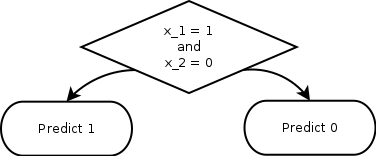
\includegraphics[scale=0.5]{3-2.png} $$
        Then, without following the decision tree algorithm, we can simplify the logic to the following,
        somitting values for convenience: \\
        \begin{verbatim}
        if x_1
            if x_2
        else
            if x_2
        \end{verbatim}


        $$ 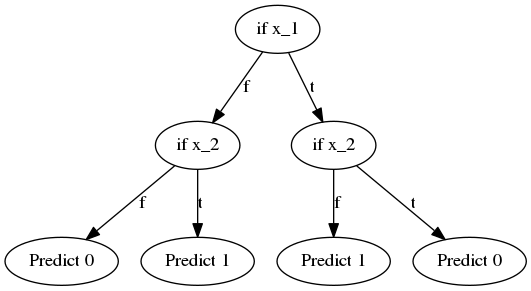
\includegraphics[scale=0.5]{3-1.png} $$
\end{enumerate}
\end{document}
